% Editable vector source. Build with: python3 gen_pipeline_svg.py
% Sized for inclusion at the manuscript's 5.5-inch text width.
% The DVI build selects dvisvgm directly, without requiring Ghostscript.
\ifdefined\SvgBuild\def\pgfsysdriver{pgfsys-dvisvgm.def}\fi
\documentclass[tikz,border=1pt]{standalone}
\usepackage[T1]{fontenc}
\usepackage{lmodern}
\usepackage{tgheros}
\usepackage{newtxmath}
\usepackage{amsmath}
\renewcommand{\familydefault}{\sfdefault}
\usetikzlibrary{arrows.meta,calc}

\definecolor{ink}{HTML}{243247}
\definecolor{muted}{HTML}{617083}
\definecolor{rule}{HTML}{D6DEE7}
\definecolor{neutral}{HTML}{F5F7FA}
\definecolor{draft}{HTML}{336BA0}
\definecolor{draftfill}{HTML}{EAF2FA}
\definecolor{target}{HTML}{B66B2E}
\definecolor{targetfill}{HTML}{FBF0E5}
\definecolor{cascade}{HTML}{39866C}
\definecolor{cascadefill}{HTML}{EDF6F1}

\newcommand{\D}{\mathcal{D}}
\newcommand{\T}{\mathcal{T}}
\newcommand{\R}{\mathcal{R}}
\newcommand{\txt}[4][]{\node[anchor=west,#1] at (#2,#3) {#4};}
\newcommand{\ctxt}[4][]{\node[#1] at (#2,#3) {#4};}
\newcommand{\card}[6]{\draw[rounded corners=5pt,fill=#5,draw=#6,line width=.75pt] (#1,#2) rectangle ++(#3,#4);}
\newcommand{\step}[4]{%
  \draw[rounded corners=3pt,fill=#3fill,draw=#3,line width=.8pt] (#1-15,#2-11) rectangle (#1+15,#2+11);
  \ctxt[text=#3]{#1}{#2}{$#4$}}
\newcommand{\lock}[2]{%
  \draw[ink,line width=.7pt] (#1-1.7,#2-.8) -- (#1-1.7,#2-2.3)
    arc[start angle=180,end angle=0,radius=1.7pt] -- (#1+1.7,#2-.8);
  \fill[ink,rounded corners=.65pt] (#1-2.7,#2-.9) rectangle (#1+2.7,#2+3.2);
  \fill[white] (#1,#2+.7) circle[radius=.65pt];}
\newcommand{\cache}[2]{%
  \foreach \i/\c in {0/target,1/draft,2/draft,3/target,4/draft,5/draft,6/#2}{
    \draw[fill=\c!27,draw=\c,line width=.6pt,rounded corners=1.3pt]
      (470+\i*12.2,#1-8) rectangle ++(10,16);
  }
  \lock{475}{#1}
  \draw[rule,line width=.6pt] (540.7,#1-10) -- (540.7,#1+10);
}

\begin{document}
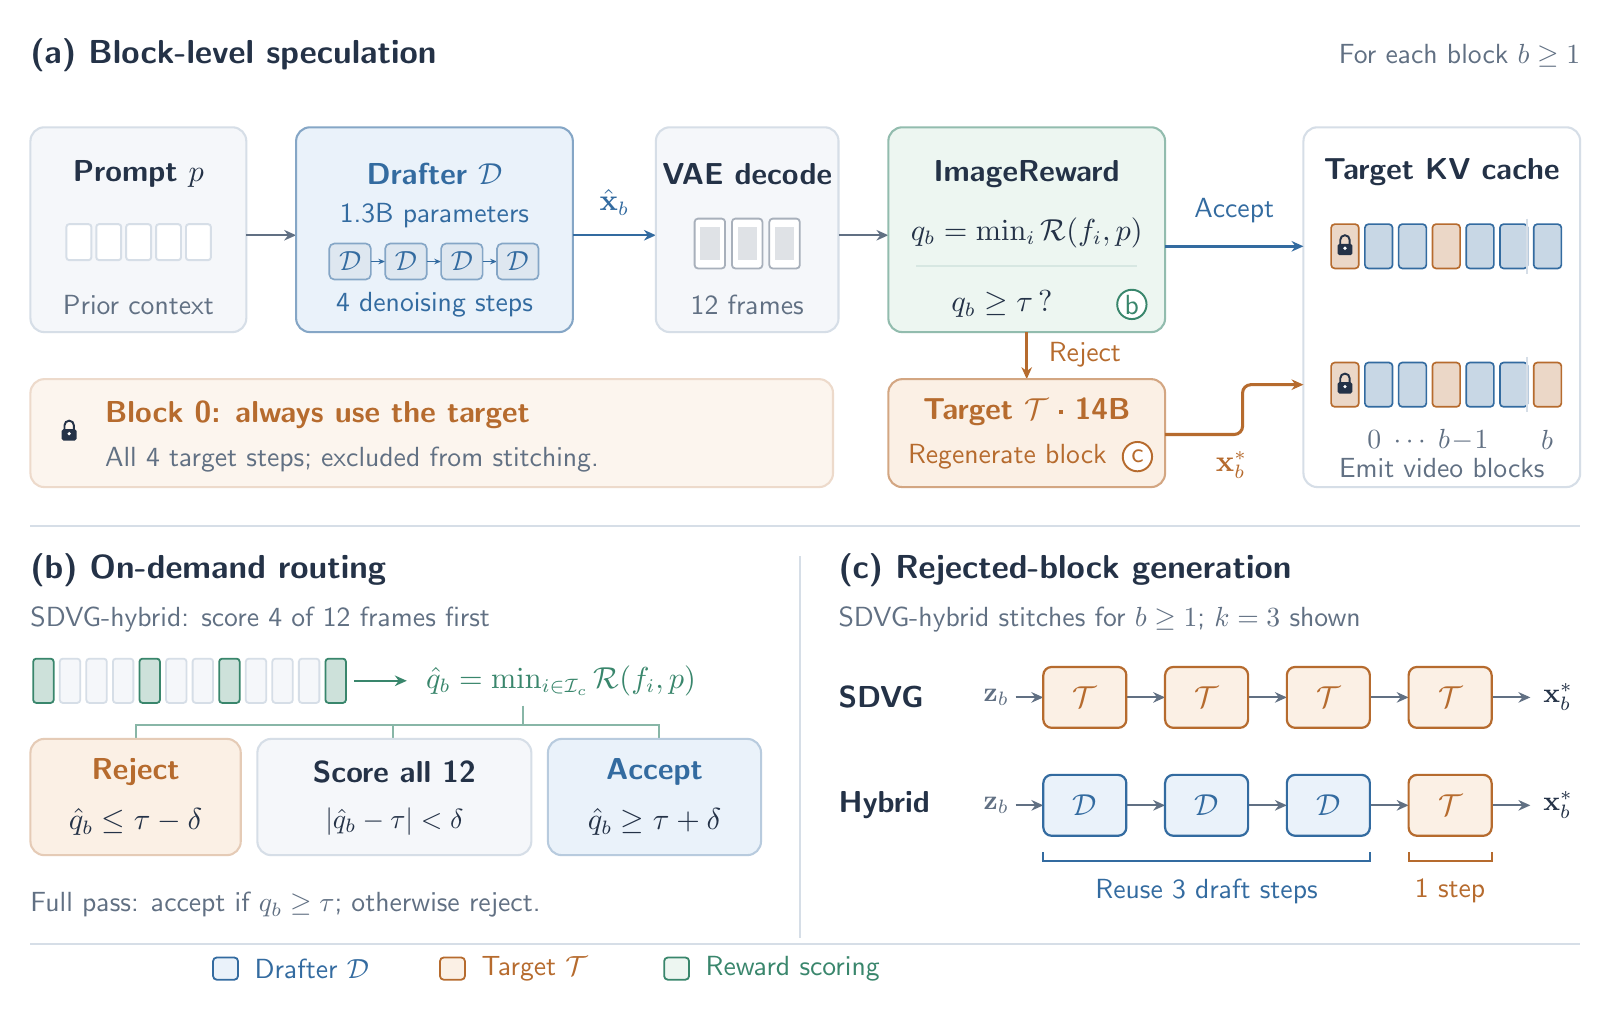
\begin{tikzpicture}[
  x=1pt,y=-1pt,
  font=\fontsize{10.5}{12}\selectfont,
  text=ink,inner sep=0pt,outer sep=0pt,
  flow/.style={-{Stealth[length=4.3pt,width=3.8pt]},draw=muted,line width=.9pt},
  dflow/.style={flow,draw=draft},
  tflow/.style={flow,draw=target},
  gflow/.style={flow,draw=cascade},
  small/.style={font=\fontsize{10}{11.5}\selectfont},
  heading/.style={font=\fontsize{12}{14}\selectfont\bfseries},
  label/.style={font=\fontsize{10.5}{12}\selectfont\bfseries}
]
\path[use as bounding box] (-1,-1) rectangle (561,347);
\fill[white] (-1,-1) rectangle (561,347);

% (a) Model-specific histories are not depicted as a single shared cache.
\txt[heading]{0}{9}{(a) Block-level speculation}
\node[anchor=east,small,text=muted] at (560,9) {For each block $b\geq1$};

\card{0}{35}{78}{74}{neutral}{rule}
\ctxt[label]{39}{52}{Prompt $p$}
\foreach \i in {0,...,4}{
  \draw[fill=white,draw=rule,rounded corners=1pt,line width=.7pt]
    (13+\i*10.8,70) rectangle ++(9,13);
}
\ctxt[small,text=muted]{39}{99}{Prior context}
\draw[flow] (78,74) -- (96,74);

\card{96}{35}{100}{74}{draftfill}{draft!60}
\ctxt[label,text=draft]{146}{52}{Drafter $\D$}
\ctxt[small,text=draft]{146}{67}{1.3B parameters}
\foreach \i in {0,...,3}{
  \draw[fill=draft!16,draw=draft!60,rounded corners=1.8pt,line width=.6pt]
    (108+\i*20.2,77) rectangle ++(15,13);
  \node[small,text=draft] at (115.5+\i*20.2,83.5) {$\D$};
  \ifnum\i<3 \draw[dflow,line width=.65pt,-{Stealth[length=2.5pt,width=2pt]}]
    (123+\i*20.2,83.5) -- ++(5.2,0);\fi
}
\ctxt[small,text=draft]{146}{99}{4 denoising steps}
\draw[dflow] (196,74) -- (226,74);
\ctxt[text=draft]{211}{62}{$\hat{\mathbf{x}}_b$}

\card{226}{35}{66}{74}{neutral}{rule}
\ctxt[label]{259}{52}{VAE decode}
\foreach \i in {0,1,2}{
  \draw[fill=white,draw=muted!55,line width=.65pt,rounded corners=1.2pt]
    (240+\i*13.5,68) rectangle ++(11,18);
  \fill[muted!20] (242+\i*13.5,71) rectangle ++(7,12);
}
\ctxt[small,text=muted]{259}{99}{12 frames}
\draw[flow] (292,74) -- (310,74);

\card{310}{35}{100}{74}{cascadefill}{cascade!55}
\ctxt[label]{360}{52}{ImageReward}
\ctxt{360}{73}{$q_b=\min_i\R(f_i,p)$}
\draw[cascade!20,line width=.6pt] (320,85) -- (400,85);
\ctxt{351}{99}{$q_b\geq\tau\,?$}
\draw[fill=white,draw=cascade,line width=.7pt] (398,99) circle[radius=5.3pt];
\ctxt[small,text=cascade]{398}{99}{b}

% Both outcomes append one block to the target cache and emit its frames.
\card{460}{35}{100}{130}{white}{rule}
\ctxt[label]{510}{51}{Target KV cache}
\cache{78}{draft}
\cache{128}{target}
\ctxt[small,text=muted]{505}{148}{$0\;\cdots\; b\! -\!1$}
\ctxt[small,text=muted]{548}{148}{$b$}
\draw[dflow,line width=1.1pt] (410,78) -- (460,78);
\ctxt[small,text=draft]{435}{65}{Accept}
\ctxt[small,text=muted]{510}{158}{Emit video blocks}

\draw[tflow,line width=1.1pt] (360,109) -- (360,126);
\txt[small,text=target]{368}{117}{Reject}
\card{310}{126}{100}{39}{targetfill}{target!60}
\ctxt[label,text=target]{360}{138}{Target $\T$\;\textperiodcentered\;14B}
\ctxt[small,text=target]{353}{154}{Regenerate block}
\draw[fill=white,draw=target,line width=.7pt] (400,154) circle[radius=5.3pt];
\ctxt[small,text=target]{400}{154}{c}
\draw[tflow,line width=1.1pt,rounded corners=3pt]
  (410,146) -- (438,146) -- (438,128) -- (460,128);
\ctxt[text=target]{434}{157}{$\mathbf{x}^{*}_b$}

% The first block is an explicit exception in both algorithms.
\card{0}{126}{290}{39}{targetfill!65!white}{target!25}
\lock{14}{145}
\txt[label,text=target]{27}{139}{Block 0: always use the target}
\txt[small,text=muted]{27}{155}{All 4 target steps; excluded from stitching.}
\draw[rule,line width=.75pt] (0,179) -- (560,179);

% (b) The gray band is an open interval; endpoints make early decisions.
\txt[heading]{0}{195}{(b) On-demand routing}
\txt[small,text=muted]{0}{213}{SDVG-hybrid: score 4 of 12 frames first}
\foreach \i in {0,...,11}{
  \def\framefill{neutral}\def\frameedge{rule}
  \ifnum\i=0 \def\framefill{cascade!25}\def\frameedge{cascade}\fi
  \ifnum\i=4 \def\framefill{cascade!25}\def\frameedge{cascade}\fi
  \ifnum\i=7 \def\framefill{cascade!25}\def\frameedge{cascade}\fi
  \ifnum\i=11 \def\framefill{cascade!25}\def\frameedge{cascade}\fi
  \draw[fill=\framefill,draw=\frameedge,line width=.65pt,rounded corners=1.1pt]
    (1+\i*9.6,227) rectangle ++(7.4,16);
}
\draw[gflow] (117,235) -- (136,235);
\txt[text=cascade]{143}{235}{$\hat q_b=\min_{i\in\mathcal I_c}\R(f_i,p)$}
\draw[cascade!60,line width=.75pt] (178,244) -- (178,251) -- (38,251) -- (38,256);
\draw[cascade!60,line width=.75pt] (178,251) -- (227,251) -- (227,256);
\draw[cascade!60,line width=.75pt] (131,251) -- (131,256);
\card{0}{256}{76}{42}{targetfill}{target!35}
\card{82}{256}{99}{42}{neutral}{rule}
\card{187}{256}{77}{42}{draftfill}{draft!35}
\ctxt[label,text=target]{38}{268}{Reject}
\ctxt{38}{286}{$\hat q_b\leq\tau-\delta$}
\ctxt[label]{131.5}{268}{Score all 12}
\ctxt[small]{131.5}{286}{$|\hat q_b-\tau|<\delta$}
\ctxt[label,text=draft]{225.5}{268}{Accept}
\ctxt{225.5}{286}{$\hat q_b\geq\tau+\delta$}
\txt[small,text=muted]{0}{316}{Full pass: accept if $q_b\geq\tau$; otherwise reject.}

% (c) Each colored box is one denoising operation, not one latent state.
% Thus k=3 means three cached D operations and one additional T operation.
\draw[rule,line width=.7pt] (278,190) -- (278,328);
\txt[heading]{292}{195}{(c) Rejected-block generation}
\txt[small,text=muted]{292}{213}{SDVG-hybrid stitches for $b\geq1$; $k=3$ shown}
\txt[label]{292}{241}{SDVG}
\txt[label]{292}{280}{Hybrid}
\ctxt[small,text=muted]{349}{241}{$\mathbf z_b$}
\ctxt[small,text=muted]{349}{280}{$\mathbf z_b$}
\foreach \y in {241,280}{
  \draw[flow,line width=.75pt] (356,\y) -- (366,\y);
  \foreach \x in {396,440,484}{
    \draw[flow,line width=.75pt] (\x,\y) -- ++(14,0);
  }
  \draw[flow,line width=.75pt] (528,\y) -- (542,\y);
  \ctxt[small]{552}{\y}{$\mathbf x_b^*$}
}
\foreach \x in {381,425,469,513}{\step{\x}{241}{target}{\T}}
\foreach \x in {381,425,469}{\step{\x}{280}{draft}{\D}}
\step{513}{280}{target}{\T}
\draw[draft,line width=.75pt] (366,297) -- (366,300) -- (484,300) -- (484,297);
\ctxt[small,text=draft]{425}{311}{Reuse 3 draft steps}
\draw[target,line width=.75pt] (498,297) -- (498,300) -- (528,300) -- (528,297);
\ctxt[small,text=target]{513}{311}{1 step}

\draw[rule,line width=.65pt] (0,330) -- (560,330);
\draw[fill=draftfill,draw=draft,rounded corners=1.3pt,line width=.65pt]
  (66,335) rectangle ++(9,8);
\txt[small,text=draft]{81}{339}{Drafter $\D$}
\draw[fill=targetfill,draw=target,rounded corners=1.3pt,line width=.65pt]
  (148,335) rectangle ++(9,8);
\txt[small,text=target]{163}{339}{Target $\T$}
\draw[fill=cascadefill,draw=cascade,rounded corners=1.3pt,line width=.65pt]
  (229,335) rectangle ++(9,8);
\txt[small,text=cascade]{244}{339}{Reward scoring}
\end{tikzpicture}
\end{document}
